\section{Übersicht der Systemarchitektur[DH]}
\setauthor{David Hauser}
\begin{figure}[h]
    \centering
    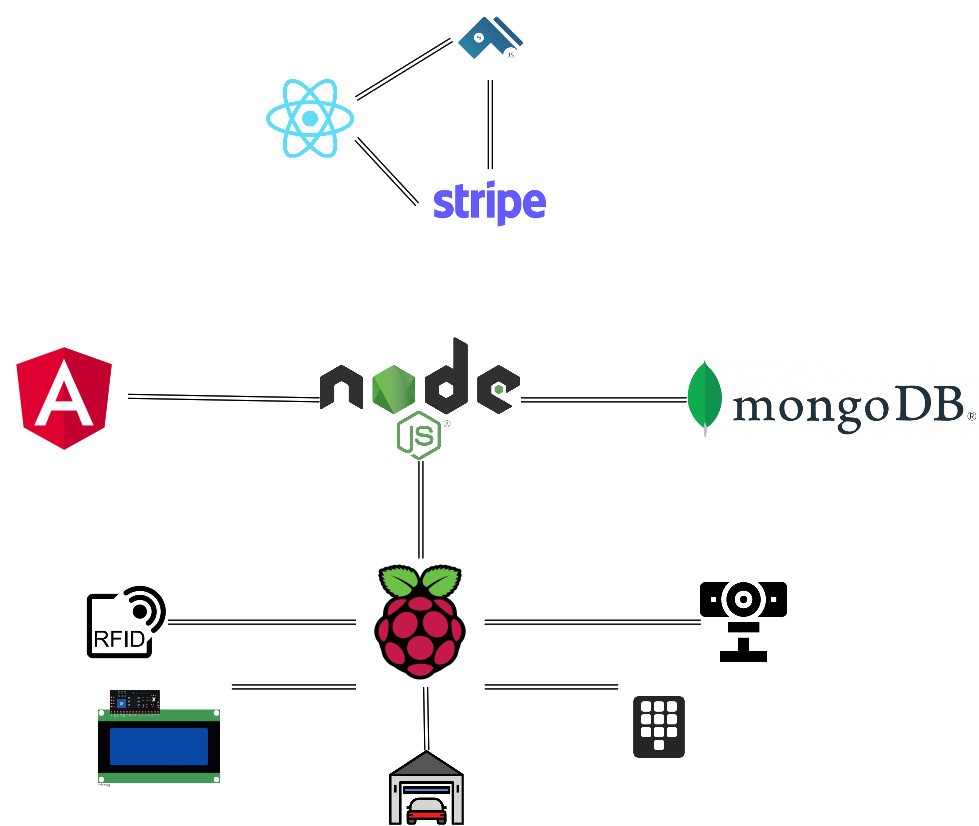
\includegraphics[width=10cm]{pics/APERTASystemarchitektur.jpg}
    \caption{Systemarchitektur}
    \end{figure}
Diese Diplomarbeit setzt sich aus zwei voneinander unabhängigen Systemen zusammen. Das Shopsystem, bestehend aus einem React-Frontend, kommuniziert mit zwei Bibliotheken, CommerceJS und Stripe, welche für die Produktverwaltung, sowie den Bezahlvorgang zuständig sind. Das Angular-Frontend des Dashboard in Verbindung mit dem NodeJS Server, der MongoDB Datenbank sowie dem Raspberry bietet das zweite System.
Der Raspberry ist über GPIOs mit dem RFID-Leser, dem Nummernfeld und dem Display verbunden. Weiters wurde die Kamera an einen der USB 3.0 Ports des Raspberry angeschlossen. Wird eine der Zutrittsmöglichkeiten positiv abgeschlossen, steuert der Raspberry Pi das Relais an, welches die Garage öffnet.
\newpage
\section{Frontend (Angular-Applikation) [DH]}
\setauthor{David Hauser}

Die Profilseite ist ein wichtiger Teil des webbasierten Clients, jedoch gibt es für die einzelnen Bauteile auch eigene Unterseiten. Auf diesen Seiten hat die Benutzerin oder der Benutzer noch mehr Möglichkeiten über die Komponenten zu entscheiden. Um die Daten für den Raspberry Pi bereitstellen zu können, werden noch weitere Funktionen benötigt.

\subsection{Aufbau von Angular}

\begin{figure}[h]
    \centering
    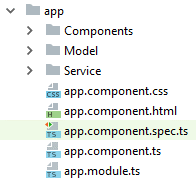
\includegraphics[width=0.4\textwidth]{pics/Aufbau_Angular.png}
    \caption{Aufbau eines Angular Projekts}
    \end{figure}

Die Applikation ist, wie bei Angular-Projekten üblich, in unterschiedliche Ordner aufgeteilt. Der App-Ordner besitzt mehrere Unterordner, welche ähnliche Funktionen gruppieren.

\subsubsection{App}
Die Dateien, welche mit app.component beginnen, werden als App bezeichnet. Sie stellen die Hauptkomponente der Angular-Applikation dar. Für das Routing im Projekt könnte noch eine app-routing.module.ts Datei angelegt werden. Wird diese nicht erstellt, kann das Routing auch in der app.module.ts durchgeführt werden. 
\pagebreak
\begin{lstlisting}[language=typescript, caption=app.module.ts]
@NgModule({
  declarations: [
    AppComponent,
    ProfileComponent,
    NfcSettingsComponent,
    KeyPadSettingsComponent,
    SignSettingsComponent,
    LoginComponent,
    NavbarComponent,
    KeypadComponent,
    SignComponent
  ],
  imports: [
    BrowserModule,
    BrowserAnimationsModule,
    [RouterModule.forRoot(routes)],
    MatCardModule,
    ReactiveFormsModule,
    MatFormFieldModule,
    MatInputModule,
    MatButtonModule,
    MatSelectModule,
    MatRadioModule,
    MatIconModule,
    HttpClientModule
  ],
  providers: [],
  exports: [RouterModule],
  bootstrap: [AppComponent]
})
export class AppModule { }
\end{lstlisting}

In dieser Datei finden die Imports der Node-Module statt. Zusätzlich werden auch die verwendeten Services importiert. Die Module werden unterteilt, um sie strukturierter zu speichern. Außerdem werden die Angular Materials Module importiert, welche der Programmiererin oder dem Programmierer helfen, die Applikation leichter zu gestalten. 

\begin{lstlisting}[language=typescript, caption=Routing der Komponenten in der app.module.ts]
const routes: Routes = [
  { path: '', component: LoginComponent },
  { path: 'profile', component: ProfileComponent },
  { path: 'nfcSettings', component: NfcSettingsComponent},
  { path: 'keyPadSettings', component: KeyPadSettingsComponent},
  { path: 'signSettings', component: SignSettingsComponent},
  { path: 'addSign', component: AddSignComponent },
  { path: 'login', component: LoginComponent},
  { path: 'nav', component: NavbarComponent}
];
\end{lstlisting}

Mittels [RouterModule.forRoot(routes)] werden die Routen innerhalb des Projekts definiert. Sie navigieren die Userin oder der User durch die einzelnen Views.

Um den Pfad einer Route zu bestimmen wird der Pfadname angegeben.  Darauf folgt die Komponente, welche aufgerufen werden soll. 

\begin{lstlisting}[caption=app.component.html]
    <app-navbar></app-navbar>
    <router-outlet></router-outlet>    
\end{lstlisting}

Diese html-Datei ist der Kern der Anwendung. Mittels <app-navbar> wird die Navbar eingebunden, welche dauerhaft am Client angezeigt wird. Im Befehl <router-outlet> werden die Komponenten, die bei den Routen im app.module.ts angegeben sind, angezeigt.

\subsubsection{Komponenten}
In diesem Ordner sind alle Komponenten auffindbar, die in der Anwendung verwendet werden. Es sind also alle Seiten mit ihren Unterkomponenten, wobei eine Seite eine gesamte Komponente darstellt, zu finden.

\subsubsection{Service}
Dieser Ordner beinhaltet alle Dienste für die Applikation. Die Funktionsweise und Verwendung wird nachfolgend noch genauer beschrieben.

\subsection{Angular-Komponente}
Die Anzeigeelemente in Angular werden als Komponenten bezeichnet. Diese werden als eigene HTML-Elemente definiert. Sie stellen abhängig von ihrer Anzeige-Logik und den Daten den Zustand der Anwendung dar.

\begin{figure}[h]
    \centering
    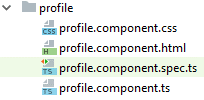
\includegraphics[width=0.4\textwidth]{pics/Aufbau_Komponente.png}
    \caption{Aufbau einer Angular Komponente}
\end{figure}
\newpage
Jede Komponente besteht aus:

\begin{itemize}
    \item HTML
    \item CSS
    \item TypeScript
    \item spec.TypeScript 
\end{itemize}

Wie sich die Komponente verhält und welche Daten sie anzeigt, wird in der TypeScript Klasse definiert. Ihr Aussehen und wo die Daten genau angezeigt werden sollen, wird in der HTML-Datei festgelegt. Ihr Design kann über das CSS-File bestimmt und beeinflusst werden.
\cite{AngularKomponenten}

\subsection{Services}
Für die Daten und Logik, welche nicht nur in einer Komponente verwendet werden, werden Angular Services genutzt. Darin werden Attribute und Methoden definiert, welche anschließend von anderen Komponenten und Services verwendet werden können.

\begin{figure}[h]
    \centering
    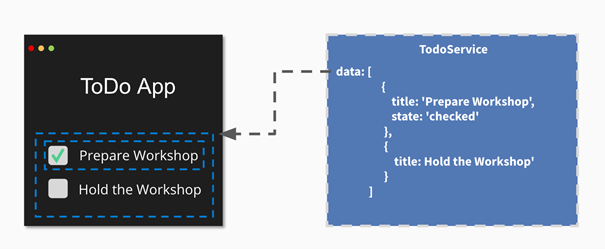
\includegraphics[width=0.8\textwidth]{pics/Service_Klasse.png}
    \caption{Auslagern einer Service Klasse}
    \cite{Service}
\end{figure}

Das Service liefert also die eigentlichen Daten für die Komponente. Die Daten gehören nicht in die Komponente. Explizite Aufgaben sollten in einem entsprechenden Service ausgelagert werden. Um die ausgelagerten Daten dann in die Komponente zu bekommen, wird Dependency Injection verwendet.
\newpage

\subsection{Dependency Injection}
Unter Dependency Injection oder auch Inversion of Control wird ein Design-Pattern verstanden. Die Dependency sollte also nicht von der aufrufenden Stelle selbst erzeugt werden. Letztere sollte die Kontrolle abgeben und nur die Abhängigkeiten definieren.

\begin{figure}[H]
  \centering
  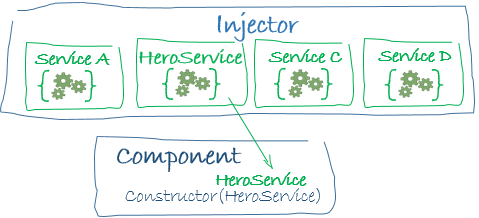
\includegraphics[width=0.6\textwidth]{./pics/DependencyInjection.png}
  \caption{Dependency Injection}
\cite{DependencyInjection}
\end{figure}
In Angular werden die verschiedenen Services vom sogenannten Injector verwaltet. Dieser gibt eine Referenz des Service und die aufrufende Stelle an, sofern dieser definiert ist. Über den Konstruktor wird die Definition der Abhängigkeit abgebildet. In einem Konstruktor können dann die Methoden des Service aufgerufen und somit auf die Daten zugegriffen werden.
\cite{AngularService}

\section{Frontend (React-Applikation) [BG]}
\setauthor{Benjamin Golic}
Die React-Applikation besteht aus mehreren Komponenten.

\subsubsection{Applikationsstruktur}
\setauthor{Benjamin Golic}

\begin{figure}[H]
  \centering
  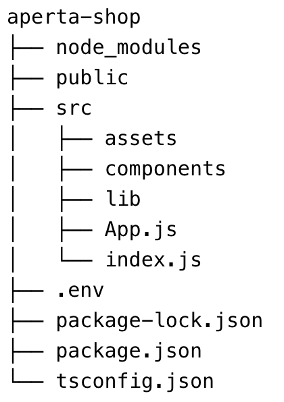
\includegraphics[width=0.2\textwidth]{pics/react-ordnerstruktur.png}
  \caption{Ordnerstruktur der React-Applikation}
\end{figure}

Grundsätzlich besteht eine React-App aus Node-Modules, einer TS-Config, einem Package-File und dem Source-Code. Das Package-File dient zur Verwaltung der Projekt-Abhängigkeiten und -Metadaten. Die TS-Config ist für die Kompilieroptionen des Projekts verantwortlich.

Des Weiteren verwenden Entwicklerinnen oder Entwickler eine „.env“-Datei in ihren Projekten. Da diese Datei sensible Daten, wie beispielsweise API-Schlüssel enthalten, werden sie nicht versioniert. Aus diesem Grund müssen die Entwickelnden die Datei lokal gespeichert haben. Die „.env“-Datei ist eine gewöhnliche Textdatei, die Umgebungsvariablen beinhaltet.
\cite{envFile}

\begin{figure}[H]
  \centering
  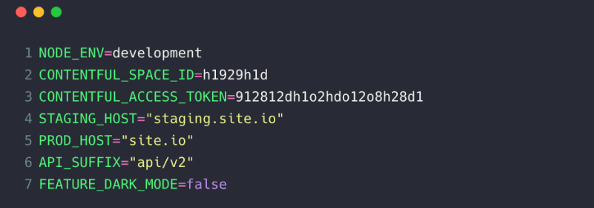
\includegraphics[width=0.8\textwidth]{pics/bsp-env.png}
  \caption{Ordnerstruktur der React-Applikation}
  \cite{envExample}
\end{figure}

\subsubsection{React-Komponente [BG]}
\setauthor{Benjamin Golic}

\begin{figure}[H]
  \centering
  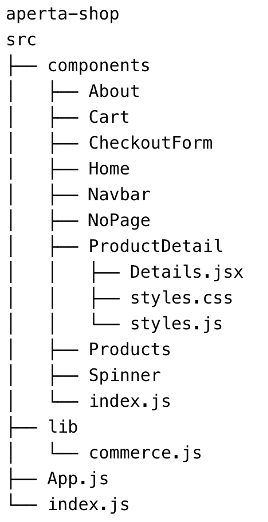
\includegraphics[width=0.3\textwidth]{pics/react-komponentenstruktur.png}
  \caption{Komponenten der React-Applikation und Aufbau der „ProductDetail“-Komponente}
\end{figure}

Grundsätzlich gibt es keine Vorgaben wie eine React-Komponente aufgebaut sein soll. Es gibt lediglich gängige Ansätze, an die sich die Entwickelnden halten können. Die zwei beliebtesten Ansätze sind die Gruppierung nach Markmalen oder Routen und die Gruppierung nach dem Dateitypen.
\cite{reactComponents}

In diesem Projekt bestehen die Komponenten aus einer „.jsx“-Datei, einer „styles.js“-Datei und meistens zusätzlich aus einer „styles.css“-Datei. Die „.jsx“-Datei ist für den Aufbau und der Logik verantwortlich. Die anderen beiden Dateien werden für die Gestaltung verwendet.

Die „App.js“-Datei ist die Haupt-Komponente der React-Applikation. Diese Komponente dient als Container für alle anderen Komponenten. Sie enthält unter anderem das Routing.
\cite{appJS}

Das Routing dient dazu, die Benutzeroberfläche mit dem URL zu synchronisieren. Es legt fest, welcher Inhalt bei welcher URL angezeigt werden soll. Es ermöglicht die Navigierung durch die Web-Applikation, ohne die komplette Seite neu laden zu müssen. 
\cite{reactRouting}

\begin{lstlisting}[language=JavaScript, caption=Source-Code des Routers, label=lst:impl:reactRouterSourceCode]
  <Router>
    <div style={{ display: 'flex' }}>
      <CssBaseline />
      <Navbar totalItems={cart.total_items} handleDrawerToggle={handleDrawerToggle} />
      <Routes>
        <Route path="/components" element={<Products products={products} onAddToCart={handleAddToCart} handleUpdateCartQty />} />
        <Route path="/packages" element={<Products products={pproducts} onAddToCart={handleAddToCart} handleUpdateCartQty />} />
        <Route path="/home" element={<Home products={pproducts} onAddToCart={handleAddToCart} handleUpdateCartQty/>} />
        <Route path="/about" element={<About />} />
        <Route path="/cart" element={<Cart cart={cart} onUpdateCartQty={handleUpdateCartQty} onRemoveFromCart={handleRemoveFromCart} onEmptyCart={handleEmptyCart} /> } />
        <Route exact path="/checkout" element={ <Checkout cart={cart} order={order} onCaptureCheckout={handleCaptureCheckout} error={errorMessage} /> } />
        <Route exact path="/" element={<Home products={pproducts} onAddToCart={handleAddToCart} handleUpdateCartQty/>} />
        <Route exact path="/detail/:id" element={<Details onAddToCart={handleAddToCart} handleUpdateCartQty />} />
        <Route path="*" element={<NoPage />} />
      </Routes>
    </div>
  </Router> 
\end{lstlisting}

\subsubsection{Gestaltung der Benutzeroberfläche}
\setauthor{Benjamin Golic}

Für die Gestaltung der Benutzeroberfläche kamen CSS und JSS zum Einsatz.

JSS ist eine JavaScript-Library, die es Entwickelnden ermöglicht, Stile auf konfliktfreie und wiederverwendbare Weise zu schreiben. Diese Bibliothek kann sowohl client- als auch serverseitig kompiliert werden. 
\cite{jss}

\begin{lstlisting}[language=JavaScript, caption=Beispiel Source-Code für die Verwendung von JSS, label=lst:impl:bspJSS]
  import jss from "jss";
  import preset from "jss-preset-default";
  
  jss.setup(preset());
  
  const styles = {
    wrapper: {
      padding: 40,
      background: "#f7df1e",
      textAlign: "center"
    },
    title: {
      font: {
        size: 40,
        weight: 900
      },
      color: "#24292e"
    },
    link: {
      color: "#24292e",
      "&:hover": {
        opacity: 0.5
      }
    }
  };
\end{lstlisting} \cite{jssExample}

Da Webapplikationen auch auf mobilen Geräten verfügbar sein sollen, muss die Benutzeroberfläche an unterschiedlichste Bildschirmgrößen angepasst werden. Hierbei wird von „Responsive Design“ gesprochen. Um dies zu realisieren, können Entwicklerinnen oder Entwickler auf bestimmte CSS-Libraries zurückgreifen. Allerdings bietet klassisches CSS „Flexbox“ und „Grid“ Möglichkeiten für die Realisierung eines Responsive Designs. Bei diesen Möglichkeiten handelt es sich um zwei signifikant unterschiedliche Layout-Technologien.
 \newpage

\subsubsection{CSS-Flexbox}
\setauthor{Benjamin Golic}

Dieses Modell bietet sich besonders für lineare Strukturen an, da es mit zwei Achsen, auf denen Inhalte verteilt werden können, arbeitet. Grundsätzlich wird hier mit einem Flex-Container und den darin enthaltenen Kind-Elementen (Flex-Items) gearbeitet. 
\cite{flexbox}

\begin{figure}[H]
  \centering
  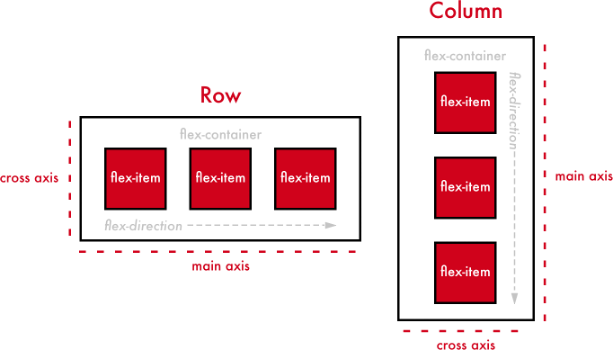
\includegraphics[width=0.8\textwidth]{pics/flexDirection.png}
  \caption{Darstellung der Flex-Direction}
  \cite{flexbox2}
\end{figure}


\begin{lstlisting}[language=HTML, caption=HTML-Code vom Aufbau einer Flexbox , label=lst:impl:flexHTML]
  <div class="flex-container">
    <div class="flex-item"></div>
    <div class="flex-item"></div>
    <div class="flex-item"></div>
    <div class="flex-item"></div>
  </div>
\end{lstlisting} \cite{flexbox}

Um die Flexbox auf dem Container-Element zu aktivieren, muss dem „flex-container“ im CSS-Code die Eigenschaft „display:flex“ zugewiesen werden. 
\cite{flexbox}

\begin{lstlisting}[language=CSS, caption=CSS-Code zur Aktivierung der Flexbox, label=lst:impl:flexCSS]
  .flex-container {
    display: flex;
  }
\end{lstlisting} \cite{flexbox}

\subsubsection{CSS-Grid}
\setauthor{Benjamin Golic}

Mit diesem Modell werden Zeilen und Spalten für einen Bereich definiert, für welche dann Elemente zugewiesen werden. Grundsätzlich wird hier mit einem Elternelement gearbeitet, in dem das Raster definiert wird. Die darin enthaltenen Kind-Elemente werden im Raster positioniert. 
\cite{cssgrid}


\begin{lstlisting}[language=HTML, caption=HTML-Code vom Aufbau eines Grids, label=lst:impl:gridHTML]
  <div class="container"> 
    <div>Element 1</div> 
    <div>Element 2</div> 
    <div>Element 11</div> 
    <div>Element 12</div> 
 </div>
\end{lstlisting} \cite{cssgrid}

Dem Elternelement wird mit Hilfe der CSS-Eigenschaft „display:grid“ mitgeteilt, dass CSS-Grids verwendet werden. 

\begin{lstlisting}[language=CSS, caption=CSS-Code zur Aktivierung des Grids, label=lst:impl:gridCSS]
.container { 
  display: grid; 
  grid-template-rows:200px 1fr 100px; 
  grid-template-columns:25% 25% 25% 25%; 
}
\end{lstlisting} \cite{cssgrid}

Mit den Eigenschaften „grid-template-columns“ und „grid-template-rows“ werden Rasterlinien festgelegt.
\cite{cssgrid}

\begin{figure}[H]
  \centering
  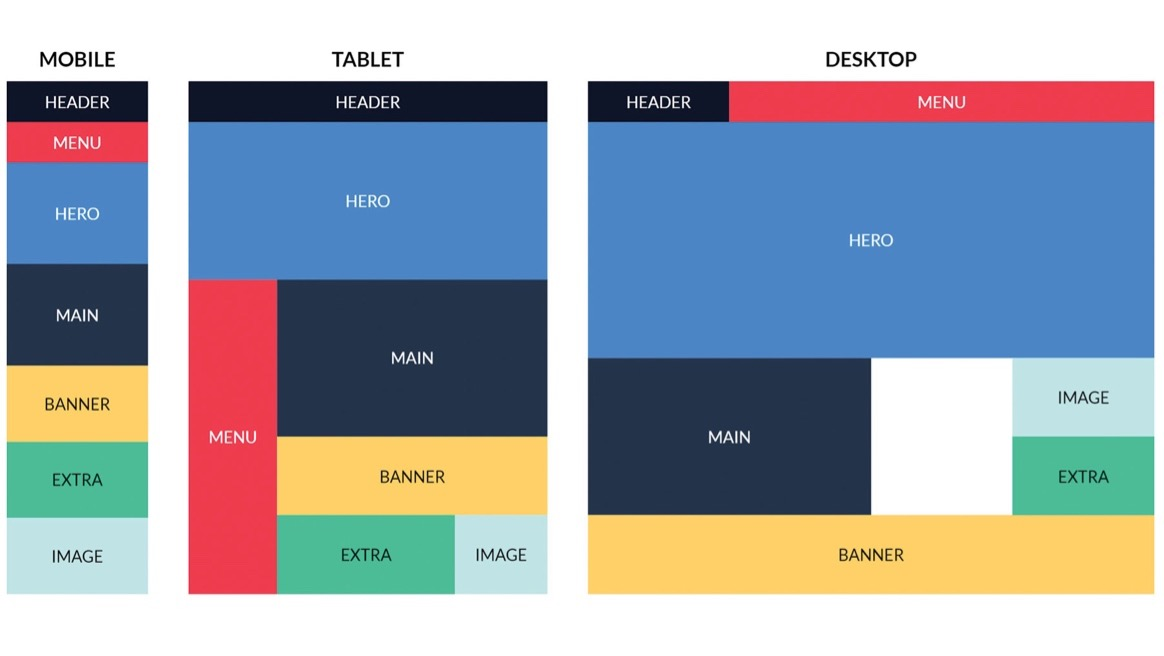
\includegraphics[width=0.6\textwidth]{pics/cssGridDarstellung.jpg}
  \caption{Darstellung eines Responsive-Designs durch CSS-Grids}
  \cite{cssgridDarstellung}
\end{figure}


\subsubsection{Commerce.js}
\setauthor{Benjamin Golic}

Commerce.js ist ein Headless-E-Commerce-Backend, welches die Integration von E-Commerce in jedes Web- und Mobil-Projekt beschleunigt. Die JavaScript-SDK und API-Suite wurden mit Fokus auf Entwickelnde entwickelt. Außerdem ermöglicht es Entwickelnden, dasselbe E-Commerce-Backend für eine Web-App und einer mobilen Anwendung zu verwenden.
\cite{commerceJS}\\

Mit Commerce.js ist es möglich eigene Produkte mit beliebigen Produktinformationen hinzuzufügen.

\begin{figure}[H]
  \centering
  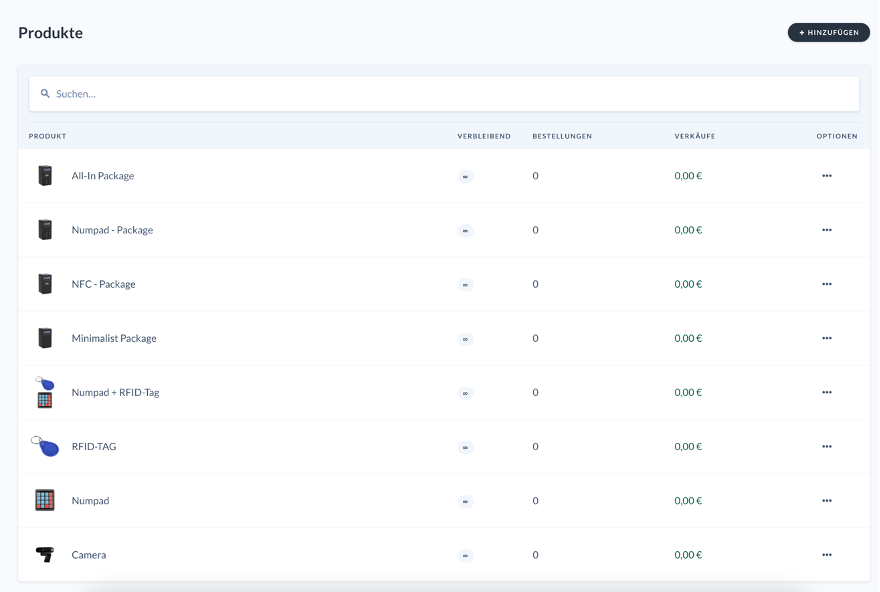
\includegraphics[width=0.9\textwidth]{pics/apertaProdukteCommerce.png}
  \caption{APERTA-Produkte in Commerce.js}
\end{figure}

Da die Nutzung des Verwaltungs-Dashboards keinen Programm-Code erfordert, ermöglicht es Content-Autoren, Fulfillment-Teams und Geschäftsinhabern die Verwaltung von Produkten, Kunden und Bestellungen.
\cite{commerceJS}

\newpage

\subsubsection{Stripe}
\setauthor{Benjamin Golic}

Stripe ist eine Online-Zahlungsabwicklungs- und Kreditkartenverarbeitungsplattform für Unternehmen. Diese Plattform ermöglicht eine sichere und effiziente Verarbeitung von Geldern per Kreditkarte oder Bank und überweist diese Gelder auf das Konto des Verkaufenden. Stripe umfasst sowohl eine Plattform für die Zahlungsabwicklung als auch ein Gateway für Kreditkartenzahlungen. Zusätzlich zu einmaligen Bezahlvorgängen bietet Stripe auch die Möglichkeit für Abonnements.

Bei einer korrekten Integration werden die vom Kaufenden eingetragenen Informationen beim Bezahlungsvorgang vom Web-Shop über die Stripe-Software gesendet. Diese überprüft, ob das zu zahlende Geld verfügbar ist und verarbeitet die Zahlung, bevor sie an das Händlerkonto gesendet wird. Nach einem erfolgreichem Zahlungsprozess erhalten Kaufende und Verkaufende eine Verkaufsbestätigung.

Falls bei einem Zahlungsvorgang etwas schieflaufen sollte, beispielsweise durch unzureichende Deckung auf dem Konto des Kaufenden, wird die Transaktion durch Stripe abgelehnt. Des Weiteren wird der Kaufende darüber benachrichtigt und bekommt die Möglichkeit, eine andere Zahlungsmethode zu verwenden.

Darüber hinaus überwacht Stripe auch betrügerische Transaktionen und blockiert alle verdächtig erscheinenden Transaktionen.

Bei Stripe ist man nicht auf eine Zahlungsart beschränkt. Es gibt eine große Auswahlmöglichkeit an viele gängigen Bezahlungsmethoden. Außerdem kann man mehrere davon aktivieren.

Des Weiteren liefert Stripe den Verkaufenden jede Menge an Statistiken und Berichten über die getätigten Verkäufe.

\cite{stripe}

\begin{figure}[H]
  \centering
  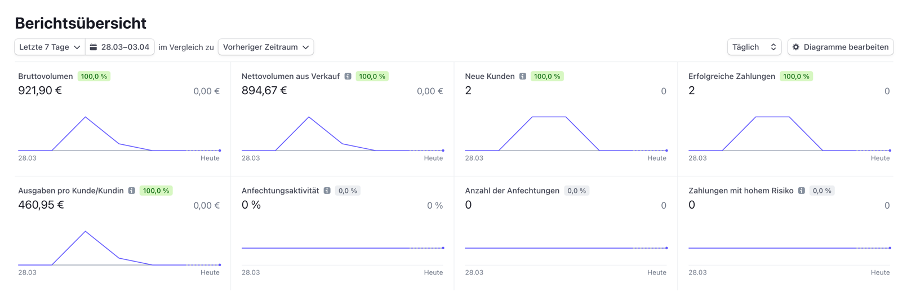
\includegraphics[width=0.9\textwidth]{pics/StripeBericht.png}
  \caption{Stripe-Berichtsübersicht}
\end{figure}